\documentclass{beamer}
\usepackage[T1]{fontenc}
\usepackage[utf8]{inputenc}

\usepackage{pgf,pgfpages}
\usepackage{tikz}
\usetikzlibrary{arrows,shapes,backgrounds,calc}

\usepackage{graphicx}
\usepackage{colortbl}
\usepackage{units}

%% Beamer style >>>>>>>>>>>>>>>>>>>>>>>>>
\mode<presentation>
{
  \usetheme{PHD}
  \setbeamercovered{transparent}
  \setbeamertemplate{items}[square]
}

%\usefonttheme[onlymath]{serif}

\beamertemplatenavigationsymbolsempty

\defbeamertemplate{enumerate item}{mycircle}
{
  %\usebeamerfont*{item projected}%
  \usebeamercolor[bg]{item projected}%
  \begin{pgfpicture}{0ex}{0ex}{1.5ex}{0ex}
    \pgfcircle[fill]{\pgfpoint{-0.1pt}{.65ex}}{1.1ex}
    \pgfbox[center,base]{\color{PHDyellow}{\insertenumlabel}}
  \end{pgfpicture}%
}
[action]
{\setbeamerfont{item projected}{size=\scriptsize}}
\setbeamertemplate{enumerate item}[mycircle]

%<<<<<<<<<<<<< beamer style

\title[DG Approximations to Anisotropic Stokes]{On stability of Discontinous Galerkin Approximations to Anisotropic Stokes Equations}
\author[J.R. Rodr\'{\i}guez Galv\'an]{\em J. Rafael Rodr\'{\i}guez Galv\'an,
  \\[1.5ex]
  \scriptsize F. Guillén González, \and M.V. Redondo Neble}
\date{\today}

% XeLaTeX font choosing
% \usepackage{fontspec}%{xltxtra} %fontspec}
% \setsansfont{Fontin Sans}
% \setsansfont{Lato}

% PDFLaTeX font choosing
\usepackage[default, scale=1.0]{lato}

% Different math fonts, see http://tug.org/pracjourn/2006-1/hartke/hartke.pdf
%\usepackage{eulervm}
%\usepackage{ccfonts, eulervm}
%\usepackage[math]{kurier}
%\usepackage[math]{anttor}
%\usepackage{pxfonts}
%\usepackage{mathpazo}
%\usepackage{mathpple}
%\usepackage[varg]{txfonts}
%\usepackage{arev}
%\usepackage{fourier}

\usepackage{tabularx}
\usepackage{array, multirow, booktabs, rotating} % booktabs: toprule, midrule...


\newcommand{\heatProblem}{(Heat-Problem)\xspace}
\newcommand{\poissonProblem}{(Poisson-Problem)\xspace}

% % Video playing
% % Commands with two or more optional arguments
% % (see http://tex.stackexchange.com/questions/29973/more-than-one-optional-argument-for-newcommand)
% \usepackage{xparse} % From future LaTeX 3
% \DeclareDocumentCommand{\PlayVideoWithLabelAutostart}{%
%   O{0.5\linewidth} O{0.5\linewidth}  O{} m }{%
%   % #1: width of video box
%   % #2: height of video box
%   % #3: Label
%   % #4: Video file
%   \begin{BoxWithVerticalLabel}{#3}{#1}
%     \href{run:#4?autostart}{\rule{#1}{#2}}
%   \end{BoxWithVerticalLabel}}

% \DeclareDocumentCommand{\PlayVideoWithNoLabelAutostart}{%
%   O{0.5\linewidth} O{0.5\linewidth} m }{%
%   \href{run:#3?autostart}{\rule{#1}{#2}}}

% \DeclareDocumentCommand{\PlayVideoNOAutoStart}{%
%   O{0.5\linewidth} O{1.0} O{} m }{%
%   \href{run:#3}{\rule{#1}{#2}}}

% \DeclareDocumentCommand{\PlayVideoWithLabelNOAutostart}{%
%   O{0.5\linewidth} O{1.0} O{} m }{%
%   \begin{BoxWithVerticalLabel}{#3}{#1}
%     \href{run:#4}{\rule{#1}{#2}}
%   \end{BoxWithVerticalLabel}}

% \DeclareDocumentCommand{\PlayVideoWithLabel}{%
%   O{0.5\linewidth} O{1.0}  O{} m }{\PlayVideoWithLabelAutostart[#1][#2][#3]{#4}}

% % \DeclareDocumentCommand{\PlayVideoWithLabel}{%
% %   O{0.5\linewidth} O{1.0}  O{} m }{\PlayVideoWithLabelNOAutostart[#1][#2][#3]{#4}}

\usepackage{presenta-granada-2018}

\newtheorem{remark}{Remark}
\newtheorem{proposition}{Proposition}
%\newtheorem{theorem}{Theorem}

% Presentation goodies >>>>>>>>>>>>>>>>>>>>>>>>>>>>
\newcommand<>{\myframed}[1]{\alt#2{\tikz[phd] \node[box] {#1};}{{#1}}}
\newcommand<>{\myframedAlert}[1]{\alt#2{\tikz[phdB] \node[boxB] {\color{black}#1};}{{#1}}}
\newcommand<>{\framedmath}[1]{%
\alt#2{\tikz[phd] \node[box] {\ensuremath{#1}};}{\ensuremath{#1}}}
\newcommand{\framedB}[1]{\tikz[phd] \node[boxB] {#1};}
\newcommand{\framedmathB}[1]{\framedB{\ensuremath{\displaystyle{#1}}}}
\newcommand{\ver}[1]{\footnote{See #1}}
\newcommand{\cita}[1]{{\color{PHDgray}\cite{#1}}}
\newcommand\cellalert[2]{\only<#1>{\cellcolor{PHDyellow}}\alt<#1>{\textbf{#2}}{#2}}
\newcommand{\soften}[1]{{\color{PHDgray}#1}}
\newcommand{\rowalert}[7]{%
    \cellalert{#1}{#2} & \cellalert{#1}{#3} &
    \cellalert{#1}{#4} & \cellalert{#1}{#5} &
    \cellalert{#1}{#6} & \cellalert{#1}{#7}}

\newcommand{\kk}{\Delta t}
% \usepackage{wasysym}
% \newcommand{\good}{{\color{PHDgreen}$\CIRCLE$}} %\blacksmiley
% \newcommand{\bad}{{\color{PHDred}$\CIRCLE$}}
\usepackage{pifont}
\newcommand{\good}{{\color{PHDgreen}\ding{52}}}
\newcommand{\bad}{{\color{PHDred}\ding{56}}}
\newcommand{\exclamation}{{\large\color{PHDred}{\textbf{\itshape !}}}}
\newcommand{\question}{{\large\color{PHDred}{\textbf{\itshape ?}}}}
\newcommand\colorUnderLine[2][PHDyellow]{\color{#1}\underline{{\color{black}#2}}\color{black}\xspace}
\newcommand\gris{\color{PHDgray}}
\newcommand\amarillo{\color{PHDyellow}}
\newcommand\tiragris[1]{{\par\hfill\small\gris{#1}}}
%<<<<<<<<<<<<<<<

\setcounter{tocdepth}{1}


%
% Bibliography
%
%\usepackage{natbib}

% To list each bibliographic entry in a line
\setbeamertemplate{bibliography entry title}{}
\setbeamertemplate{bibliography entry location}{}
\setbeamertemplate{bibliography entry note}{}

% ... end of preamble.

%======================================================================
\begin{document}
%======================================================================

% Tikz style and beamer template ------->>>
\tikzstyle{every picture}+=[remember picture]
\tikzstyle{na} = [baseline=-.5ex]
\tikzstyle{phd} = [baseline=-.6ex,
  box/.style={rectangle, draw=PHDblueC, thick, fill=PHDblueA,
    align=center, rounded corners, minimum height=1.6em},
  boxB/.style={rectangle, draw=PHDredA, thick, fill=PHDblueA,
    align=center, rounded corners, minimum height=1.6em}]
\tikzstyle{phdB} = [baseline=-.7ex,
  box/.style={rectangle, draw=PHDblueC, thick, fill=PHDblueA,
    align=center, rounded corners, minimum height=1.6em},
  boxB/.style={rectangle, draw=PHDredA, thick, fill=PHDblueA,
    align=center, rounded corners, minimum height=1.6em}]
\tikzstyle{myarrow} = [->,>=latex, PHDredA, shorten >=4pt,
  opacity=.6, line width=0.6mm]
\tikzstyle{myarrow2} = [->,>=latex, PHDblueC, shorten >=4pt, opacity=.2, line width=0.4mm]
\tikzstyle{myarrow3} = [
     opacity=.7,
%    >=triangle 60,              % Nice arrows; your taste may be different
    node distance=6mm and 60mm, % Global setup of box spacing
    every join/.style={norm},   % Default linetype for connecting
                                % boxes
    line width=0.6mm,
    PHDredA,
    ->
    ]
\setbeamertemplate{background}
 {
\includegraphics[width=\paperwidth,height=\paperheight]{frontpage_bg}}
\setbeamertemplate{footline}[default]
% <<<-------


% Write custom titlepage ------->>>
\begin{frame}
  \titlepage
  \vspace{5cm}
\end{frame}

% Set the background for the rest of the slides.
\setbeamertemplate{background}
 {
\includegraphics[width=\paperwidth,height=\paperheight]{slide_bg}}


% Write all of the slides..........

\begin{frame}{Outline}
  \tableofcontents
\end{frame}

% Start inserting infoline at the end
\setbeamertemplate{footline}[PHDtheme]
% <<<-------

\newcommand{\imgdir}{Undefined, use renewcommand!}

%%,---------------------------------------------------------------------
%%| Introduction
%%`---------------------------------------------------------------------
\section[Introduction]{Stability of Anisotropic Stokes Equations}
\label{sec:introduction}

\begin{sectionframe}
\end{sectionframe}

\begin{frame}{Anisotropic equations for (large scale) ocean}
%----------------------------------------------------------------------
  \begin{itemize}\itemsep0.5em
  \item<1> \structure{The ocean:} A slightly compressible fluid
    endowed with Coriolis and buoyancy forces and a set of
    conservation laws from
    Physics
  \item<2-> Simplification of physical laws:\vspace{-1em}
    \begin{columns}
      \column{0.05\linewidth}
      \column{0.41\linewidth}
      \begin{enumerate}\itemsep1.5em
      \item<2-> Boussinesq hypothesis
        \tikz[na] \coordinate(Lboussinesq);
        \hfill
        \tikz[na] \coordinate(Rboussinesq);
      \item<3-> Cartesian coordinates
        \tikz[na] \coordinate(LbetaPlane);
        \hfill
        \tikz[na] \coordinate(RbetaPlane);
      \item<4-> Vertical scaling
        \tikz[na] \coordinate(LverticalScaling);
        \hfill
        \tikz[na] \coordinate(RverticalScaling);
      \end{enumerate}
      \column{0.54\linewidth}
      \begin{overprint}
        \onslide<2>
        \begin{block}{Boussinesq Hypothesis}
          \begin{itemize}
          \item \textit{Density} does not depart from a \textit{mean reference value},
            $\rho_\star>0$
          \item Hence density can be replaced by the constant
            $\rho_\star$ except in
            % \begin{itemize}
            % \item
              \textit{buoyancy} term
            % \item conservation of \textit{energy equation}
              {\color{PHDgrayC} (and state equation)}
          \end{itemize}
        \end{block}
        \onslide<3>
        \begin{block}{Cartesian Coordinates}
          \begin{itemize}
          \item A \textit{local projection} of the Earth surface will be
            assumed
          \item \textit{No loss of generality}: spherical coordinates requires
            only the proper handling of some terms
          \end{itemize}
        \end{block}
        \onslide<4>
        \begin{block}{Vertical Scaling of Domain}
          \vspace{-0.5em}
          \begin{itemize}
          \item The \textit{aspect ratio}
            \begin{equation*}
              \framedmath{\displaystyle\varepsilon = \frac{\text{vertical
                    scales}}{\text{horizontal scales}}}~
                \begin{tabular}[t]{l} is \large\textbf{small} \\[-0.2ex]
                  \tiny\it ~ $10^{-3}$, $10^{-4}$\end{tabular}
            \end{equation*}
%            \pause
          \item \scriptsize \emph{Physical} point of view: dominant terms in
            \textit{vertical momentum} equation
          \item \emph{Numerical} point of view: the problem is
            \textit{rescaled}, obtaining...
            \begin{itemize}
            \item \alert{\textbf{Isotropic domain}}
            \item \alert{\textbf{Anisotropic equations}}
            \end{itemize}
          \end{itemize}
        \end{block}
      \end{overprint}
    \end{columns}
  \end{itemize}
\end{frame}

%----------------------------------------------------------------------
\begin{frame}{Isotropic domain}
%----------------------------------------------------------------------
%  \vspace*{0.5em}
 After geometrical scaling, we obtain:
   $$
   \domain = \bigl\{ (\xx,z)\in \Rset^{3} \ /\ \xx=(x,y)\in\surface,\
   -D(\xx)< z < 0 \bigr\},
   $$
   where $\surface\subset\Rset^{2}$ is surface domain and
   $D:\overline\surface \to \Rset_{+}$ is depth function
   \begin{center}
     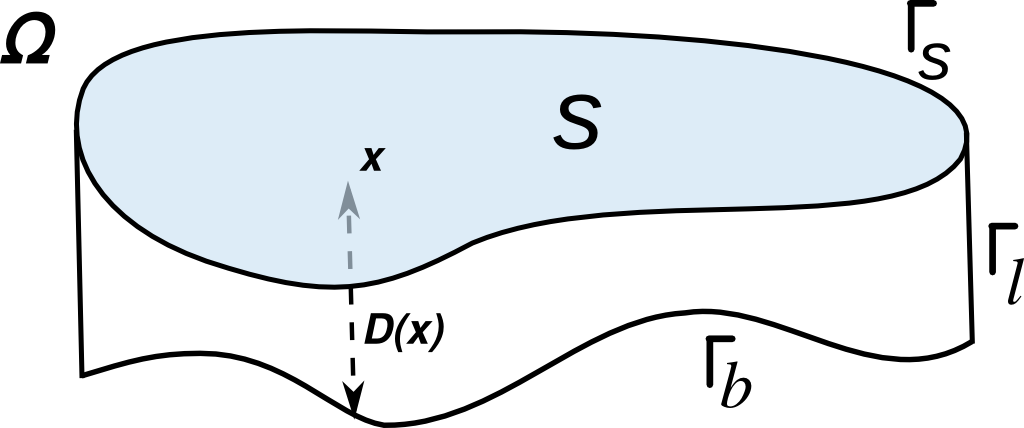
\includegraphics[width=0.4\textwidth]{img/domain}
   \end{center}
   \begin{itemize}
     \setlength\itemsep{1em}
   \item \alert{Rigid lid hypothesis} (flat surface) is introduced
   \item
     \color{darkgray} Notation:
     \begin{itemize}
     \item \color{darkgray} $\surfaceBoundary$: part of the boundary corresponding to
       the surface
     \item \color{darkgray} $\bottomBoundary$: part corresponding to the bottom
       boundary
     \item \color{darkgray} $\talusBoundary$: lateral walls (if any)
     \end{itemize}
   \end{itemize}
 \end{frame}

%----------------------------------------------------------------------
\begin{frame}{Anisotropic equations}
%----------------------------------------------------------------------
%  \vspace{-0.2em}
  \note{Comment briefly the main difficulties of Navier-Stokes equations}
  \begin{overprint}
    \onslide<1>
    Anisotropic momentum equations (in the isotropic) domain:
    \onslide<2>
    \alert{Vertical/Horizontal aspect ratio} \tikz[na] \coordinate(LaspectRatio);
    \  affects vertical velocity terms!
    \onslide<3>
    \alert{Coriolis} force
    \tikz[na] \coordinate(Lcoriolis);
    \onslide<4>
    \alert{\textbf{Density}}: \textbf{coupling} of energy equations.
    \tikz[na] \coordinate(Lcoupling);
    \onslide<5>
    \textbf{We focus on \dotfill \alert{Constant density case}}
    \onslide<6>
    \textbf{We focus on \dotfill \alert{Linear steady case}}
  \end{overprint}
  \begin{block}{\small Conservation of momentum and continuity}
    \vspace{-0.66\baselineskip}
    \begin{align*}
      {\onslide<1-5> \dt \uu + \uu\cdot\gradx\uu + \vv\,\dz\uu  {\onslide<-6>- \visc\Delta\uu
      +}} {\onslide<1-4>\frac 1 \rho_\star} \onslide<-6> \gradx \pp=
       \tikz[na] \node (Rcoriolis) {\framedmath<3>{\fU}};
      \\
      \tikz[na] \coordinate(RaspectRatio);
        \framedmath<2>{ \varepsilon^2 \Big( {\onslide<1-5> \dt \vv + \uu\cdot\gradx\vv +
          \vv\,\dz\vv} {\onslide<-6> - \visc\Delta\vv \Big) }}
        \displaystyle
        + {\onslide<1-4> \frac 1 \rho_\star } {\onslide<-6> \dz \pp} +
        {\onslide<1-4> \frac{1}{\rho_\star}} \tikz[na] \coordinate(RcouplingA);
          \framedmath<4>{\rho}\,\gravity {\onslide<-6> = 0\hskip+0.5em}
      \\[-0.2em]
      \div\uu + \dz\vv = 0\hskip+0.5em
    \end{align*}
    \vspace{-1.4\baselineskip}
  \end{block}
  \begin{block}<4>{\small Convection-diffusion of \textit{temperature} and
      \textit{salinity} + state equation (density)}
    \vspace{-0.66\baselineskip}
    \begin{align*}
      \dt \Te  + (\uu \cdot \gradx) \Te + (\vv\cdot\dz) \Te  - \nu_\Te\Delta \Te &= \fT
      \\[0.3em]
      \dt \Sa  + (\uu \cdot \gradx) \Sa + (\vv\cdot\dz) \Sa -
      \nu_\Sa\Delta \Sa &= \fS
      \\[0.3em]
      \tikz[na] \coordinate(RcouplingB);
      \framedmath<4>{\rho} = \rho_\star\big(1-\beta_\Te(\Te-\Te_\star) + \beta_\Sa(\Sa&-\Sa_\star)\big)
    \end{align*}
    \vspace{-1.4\baselineskip}
  % \item Equation of state (dependence of density in terms of
  %   temperature and salinity)
  %   where $\Te_\star$ and $\Sa_\star$ are given reference values.
  \end{block}
  \tikzstyle{RaspectRatio} = [draw, circle, minimum size=.5cm, node
  distance=1.75cm]
  \tikzstyle{redcircle} = [draw, circle, color=PHDredA, node distance=3cm,
  minimum height=2em]

  \begin{tikzpicture}[overlay]
    \path<2>[myarrow]
    (LaspectRatio) edge [out=320, in=130] (RaspectRatio);
    \path<3>[myarrow]
    (Lcoriolis) edge [out=0, in=130] (Rcoriolis);
    \path<4>[myarrow]
    (Lcoupling) edge [out=0, in=135] (RcouplingA);
    \path<4>[myarrow]
    (Lcoupling) edge [out=0, in=135] (RcouplingB);
        % \draw<3>[->, PHDblue, ultra thick, opacity=.8] (Lboussinesq) -- (Rboussinesq);
        % \draw<4>[->, PHDblue, ultra thick, opacity=.8] (LbetaPlane) -- (RbetaPlane);
        % \draw<5>[->, PHDblue, ultra thick, opacity=.8] (LverticalScaling) -- (RverticalScaling);
  \end{tikzpicture}
\end{frame}

%--------------------------------------------------------------------------
\begin{frame}{Steady Anisotropic Stokes equations}
%--------------------------------------------------------------------------
  \color{darkgray}{\small Thus we are interested in numerical resolution of:}
  \bigskip
  \begin{center}\large
    \textit{mixed anisotropic velocity/pressure problems}
  \end{center}
  \bigskip
  \begin{center}
    \uncover<2>{... when $\framedmath<2>{\varepsilon\to 0}$}
  \end{center}
  \begin{block}{Steady Anisotropic Stokes equations}
    \begin{equation*}
      \begin{aligned}
        - \nu\Delta\uu + \gradx\pp &= \ff,
        \\
        \framedmath<2>{-\varepsilon^2 \Delta\vv} + \dz\pp &= 0,
        \\
        \divx\uu + \dz\vv &= 0.
      \end{aligned}
    \end{equation*}
  \end{block}
\end{frame}


%--------------------------------------------------------------------------
\begin{frame}{Not Easy Task!}
%--------------------------------------------------------------------------
  \begin{center}
      \begin{tabular}[b]{r}
        $\P2/\P1$ F.E.
        \\[1ex]
        Velocity
        \\[1ex]
        \alert{$\framedmath{\varepsilon=10^{-2}}$}
        \\
        \rule{0pt}{0.5\textheight}
      \end{tabular}
      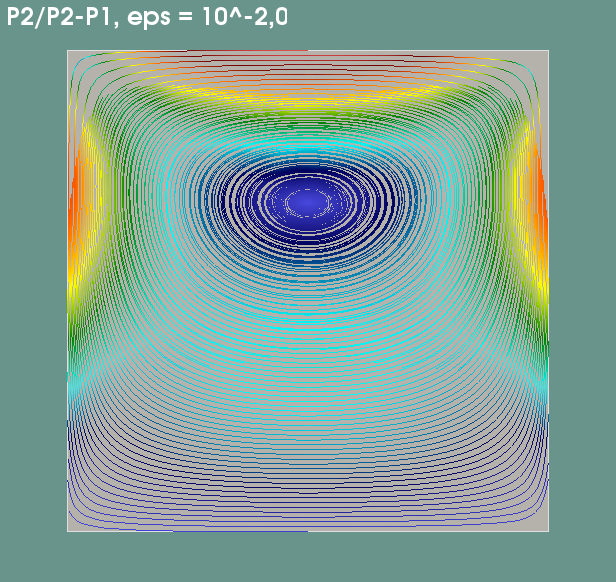
\includegraphics[width=0.7\linewidth]{img/221-eps-2}
  \end{center}
\end{frame}

%--------------------------------------------------------------------------
\begin{frame}{Not Easy Task!}
%--------------------------------------------------------------------------
  \begin{center}
      \begin{tabular}[b]{r}
        $\P2/\P1$ F.E.
        \\[1ex]
        Velocity
        \\[1ex]
        \alert{$\framedmath{\varepsilon=10^{-3}}$}
        \\
        \rule{0pt}{0.5\textheight}
      \end{tabular}
      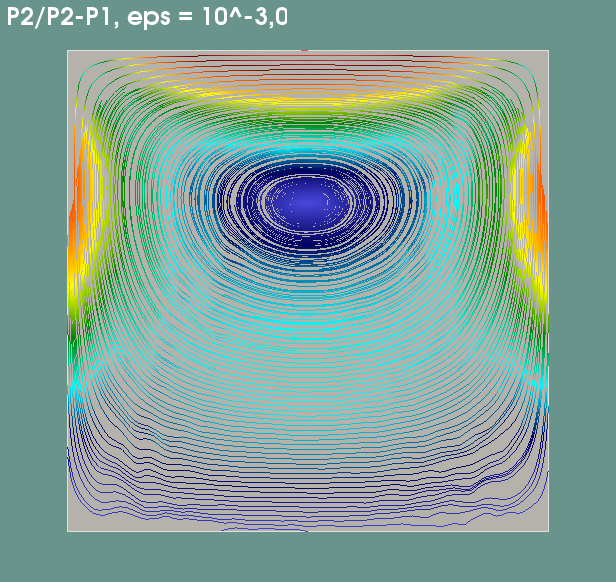
\includegraphics[width=0.7\linewidth]{img/221-eps-3}
  \end{center}
\end{frame}

%--------------------------------------------------------------------------
\begin{frame}{Not Easy Task!}
%--------------------------------------------------------------------------
  \begin{center}
      \begin{tabular}[b]{r}
        $\P2/\P1$ F.E.
        \\[1ex]
        Velocity
        \\[1ex]
        \alert{$\framedmath{\varepsilon=10^{-4}}$}
        \\
        \rule{0pt}{0.5\textheight}
      \end{tabular}
      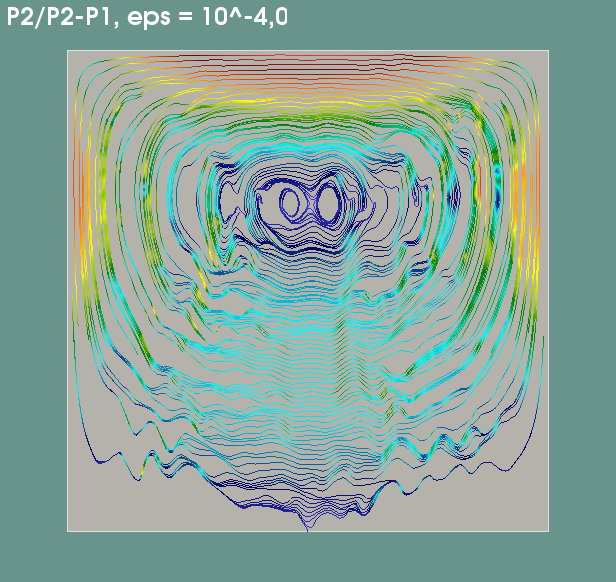
\includegraphics[width=0.7\linewidth]{img/221-eps-4}
  \end{center}
\end{frame}

%--------------------------------------------------------------------------
\begin{frame}{Instability of \textit{Classical} Finite Elements}
%--------------------------------------------------------------------------
  \begin{itemize}
    \itemsep=1.2em
  \item ``Classical'' Taylor-Hood $\P2/\P1$ F.E. \textbf{not stable} when $\varepsilon\to 0$
  \item Similar results for bubble $\P{1,b}/\P1$ F.E.
  \item Why? \ \ One has stokes-like inf-sup condition...
    \par\hfill\uncover<2->{\alert<2>{and also a \textbf{new hydrostatic inf-sup condition}}}
    \begin{alignat*}{4}
      \label{eq:ISp}
      \tag*{\ensuremath{(IS)^\PP}\xspace}
      &\quad&
      \sup_{0\neq(\uu,\vv)\in \UU \times \VV}
      \frac{(\div(\uu,\vv),\pp)}{\|\grad \uu,\dz \vv\|}
      &\ge \ConstISp \|\pp\|
      &\quad&
      \forall \pp \in \PP,
      \\[1.0em]
      \label{eq:ISv}
      \onslide<2->
      \tag*{\ensuremath{(IS)^\VV}\xspace}
      &\quad &
      \alert<2>{
        \sup_{0\neq \pp \in \PP}
        \frac{(\dz \vv,\pp)}{\|\pp\|}}
      &\alert<2>{\ge \ConstISv \|\dz\vv\|}
      &\quad&
      \alert<2>{\forall \vv\in \VV}
    \end{alignat*}
  \item<3> New inf-sup condition means:
    \begin{center}
      \structure{\# dofs($\alert{v}$)} not bigger than \structure{\#
        dofs($\alert{p}$)}
    \end{center}
  \end{itemize}
\end{frame}

%---------------------------------------------------------------------
\begin{frame}{How to proceed?}
%---------------------------------------------------------------------
  \begin{description}
    \itemsep=1.5em
  \item[Idea 1] To introduce \textbf{new \emph{anisotropic} F.E.}~\cite{fguillen-rrgalvan-paper2-NumMath:2015,fguillen-rrgalvan-paper1-ApNumMath:2016}
    \begin{flushright}\it
      (which verify~\ref{eq:ISp} and also~\ref{eq:ISv})
    \end{flushright}
  \item[Idea 2] To introduce \textbf{new \emph{stabilized} schemes}~\cite{fguillen-rrgalvan-paper3-SIAM:2015}
    \begin{flushright}\it
      (which do not require~\ref{eq:ISv})
    \end{flushright}
  \item<2>[Idea 3] To \myframed{\textbf{Explore Discontinuous Galerkin F.E.}}
    \begin{flushright}\it
      (which, in some sense, verify~\ref{eq:ISp} and also~\ref{eq:ISv})
    \end{flushright}
  \end{description}
\end{frame}

\section[DG Formulation]{SIP DG Formulation for Anisotropic Stokes}
\label{sec:dg-formulation}

\begin{sectionframe}
\end{sectionframe}

%---------------------------------------------------------------------
\begin{frame}{Notation}
%---------------------------------------------------------------------
  \begin{itemize}
    \itemsep=0.95em
  \item \structure{$\Th$}: family of meshes of the domain $\Omega\subset\Rset^d$
  \item For instance, simplicial elements \structure{$K$} satisfying usual
    regularity:
    $$
    \exists \rho>0 \ /\ \rho\, h_K \le r_K \quad \forall K\in\Th,
    $$
  \item \structure{$\Eh$}: set of faces (edges in $2D$)\quad
    \llaveizq{\structure{$\Ehi$}: interior faces,\\[0.3em] \structure{$\Ehb$}: boundary faces}
  \item If $e=K^+\cap K^-\in\Ehi$ \llaveizq{jump: $\structure{\jump{u}_e}:= u|_{K^+}-u|_{K^-}$, \\[0.4em]
   mean: $\structure{\average{u}_e} := \frac12 (u|_{K^+}+u|_{K^-})$}
 \medskip
 \begin{itemize}
 \item[$\star$] If $e\in\Ehb$: $\jump{u}_e:= \average{u}_e:= u_e$
 \end{itemize}
\end{itemize}
\end{frame}

%---------------------------------------------------------------------
\begin{frame}{Notation II}
%---------------------------------------------------------------------
  \begin{itemize}
    \itemsep=0.95em
  \item \textit{Broken} Sobolev space:
    \begin{equation*}
      \structure{H^m(\Th)} := \big\{ u\in L^2(\Omega) \ |\ u\in H^m(K)\ \forall K\in\Th \big\},
    \end{equation*}
  \item Broken gradient operator \structure{$\gradh$}:
    $\forall u\in H^1(\Th)$,
    $$
    (\gradh u)|_K=\grad(u|_K)\quad \forall\, K\in\Th
    $$
  \item Discontinous finite-dimensional subspace of $H^m(\Th)$:
    $$
    \structure{\Pd h^k}:=
    \left\{
      u\in L^2(\Omega) \ | \ u\in \Polin{k}(K), \ \forall K\in\Th \right \}.
    $$
  \end{itemize}
\end{frame}

%---------------------------------------------------------------------
\begin{frame}{SIP (Symmetric Interior Penalty) Bilinear Form}
% ---------------------------------------------------------------------
  \textbf{\itshape Poisson problem} (homogeneous Dirichlet b.c.)
  % \vspace{-1em}
  \begin{center}
    + integration by parts in each element
    \small\cite{arnold_interior_1982,di_pietro_ern_2012}
    \quad
    $\leadsto$
  \end{center}
  \vspace{-1em}
  \begin{multline*}
    \asip[sip,\alert<3>{\eta}](\uh,\buh) = \int_\Omega \gradh \uh \cdot\gradh\buh
    \\
    \framedmath<2>{\displaystyle - \sum_{e\in\Eh} \int_e\big( \average{\gradh \uh}\cdot \nn_e \jump{\buh}
      + \jump{\uh} \average{\gradh\buh}\cdot \nn_e \big)
    }
    \\
    + \framedmath<3>{\displaystyle\alert<3>{\mathbf{\eta}}\sum_{e\in\Eh} \frac1{h_e} \int_e \jump{\uh}\jump{\buh}},
    \quad \forall\,\uh,\buh\in \Pd h^k
  \end{multline*}
  \vspace{-1em}
  \begin{itemize}
  \item<2> \myframed{Consistency and symmetry}
  \item<3> \myframed{Coercivity (for $\alert<3>{\mathbf{\eta}>0}$ big enough)}
  \end{itemize}
\end{frame}

%---------------------------------------------------------------------
\begin{frame}{SIP (Symmetric Interior Penalty) Bilinear Form II}
  % ---------------------------------------------------------------------
  \begin{definition}[SIP norm]
    \begin{equation*}
      \normsip{u} = \big(\, \norm[]{\gradh u}^2 + \seminormU{u}^2 \;\big) ^{1/2},
    \end{equation*}
    where
    \begin{equation*}
      \seminormU{u} =
      \Big (\sum_{e\in\Eh} \frac1{h_e} \int_e {\jump u}^2 \Big ) ^{1/2} \quad \text{(\textit{jump seminorm})}.
    \end{equation*}
  \end{definition}
  \begin{lemma}[Coercivity and Continuity]
    \begin{itemize}
    \item Exists $C(\eta)>0$ such that
      \begin{equation*}
        \asip[sip,\eta](\uh,\uh) \ge C(\eta) \normsip{\uh}^2, \quad \forall\,\uh\in \Pd h^k
      \end{equation*}
    \item Exists $ C_{\text{bnd}}>0$ such that
      \begin{equation*}
        \label{eq:sip:boundedness}
        \asip[sip,\eta](\uh,\buh) \le C_{\text{bnd}} \normsip{\uh}\normsip{\buh}, \quad \forall\,\uh,\buh\in \Pd h^k
      \end{equation*}
    \end{itemize}
  \end{lemma}
  \begin{flushright}
    \scriptsize \textbf{Proof}: see e.g.\cite{di_pietro_ern_2012}
  \end{flushright}
\end{frame}

%---------------------------------------------------------------------
\begin{frame}{DG Bilinear Form for Anisotropic Stokes}
% ---------------------------------------------------------------------
  \medskip
  \small
  % \begin{itemize}
    % \itemsep=1em
  % \item
  \structure{\bf Order \underline{$k$} polynomials for \underline{\textit{velocity}} and \underline{\textit{pressure}}}: \llaveizq{$\wwh=(\uuh,v_h)\in\WWh$, \\
    $\ph \in \Ph$,}
    \begin{align*}
      \WWh&=\UUh\times\Vh=(\Pd h^k)^d, \quad \UUh = (\Pd h^k)^{d-1}, \quad \Vh=\Pd h^k
      \\
      \Ph &= \Pd h^k.
    \end{align*}
    % For each $\wwh=(\uuh,\vh)$ and $\bwwh=(\buuh,\bvh) \in\WWh$, with
    % $\uuh=(u_i)_{i=1}^{d-1}$ and $\buuh=(\overline u_i)_{i=1}^{d-1}$,
  % \item
    \medskip
    \structure{\bf Anisotropic velocity bilinear form}: \enspace
    $\forall \wwh=(\uuh,\vh),\ \bwwh=(\buuh,\bvh) \in\WWh$,
    \begin{equation*}
      a_h(\wwh,\bwwh) = \Big( \sum_{i=1}^{d-1} \asip[sip , \eta](u_i,\overline u_i)
      + \tikz[na] \node(Laepsilon){\framedmath<2>{\alert<2>{\asip[\varepsilon](\vh,\bvh)}}};
      \Big),
    \end{equation*}
    \vspace{-0.5em}
    \onslide<2>
    where
    \begin{multline*}
      \alert{\framedmath<2>{\asip[\varepsilon](\vh,\bvh)} =\tikz[na] \coordinate (Raepsilon);}
      \\
      \alert{ \varepsilon \,\asip[sip, 0](\vh,\bvh)
      + \eta\sum_{e\in\Eh} \frac1{h_e} \int_e \Big( \varepsilon
      \jump{\vh\nx}\jump{\bvh\nx} + \jump{\vh\nz}\jump{\bvh\nz} \Big),}
    \end{multline*}
    \begin{itemize}
    \item[$\star$] \scriptsize $\varepsilon$--dependent bilinear form,
      standard $\vh$ SIP stabilizing term is replaced by anisotropic term
    \item[$\star$] Generalization of previous works (for Isotropic \&
      Hydrostatic viscous
      fluids~\cite{Guillen-RedondoNeble-RGalvan:17})
    \end{itemize}
  \begin{tikzpicture}[overlay]
    \path<2>[myarrow] (Laepsilon) edge [out=210, in=40] (Raepsilon);
  \end{tikzpicture}
\end{frame}

%---------------------------------------------------------------------
\begin{frame}{Partial $\varepsilon$--dependent Coercivity}
% ---------------------------------------------------------------------
  \begin{itemize}
    \itemsep=1em
  \item For \underline{$\uuh$}, coercivity of SIP bilinear form yields:
    \begin{equation*}
      \sum_{i=1}^{d-1} \asip[sip , \eta](u_i,\overline u_i) \ge
      C(\eta) \normsip{\uuh}^2 \quad
      \structure{\scriptsize=\quad C(\eta) \sum_{i=1}^{d-1}\normsip{u_i}^2}
    \end{equation*}
  \item
    For \underline{$(\uuh,\vh)$} we can show:
    \begin{lemma}[$\varepsilon$--dependent coercivity]
      For all $\eta>\eta_*$ and for all $\wwh=(\uuh,\vh) \in \WWh$,
      \begin{equation*}
        a_h(\wwh,\wwh) \ge C(\eta) \Big(
        \normsip{\uuh}^2
        + \varepsilon  \norm[0]{\gradh\vh}^2
        % + C_{\eta}^{\varepsilon}\seminormVeps{\vh}^2
        + \seminormVeps{\vh}^2
        \Big),
      \end{equation*}
      where
      $$
      \seminormVeps{\vh}^2 = \sum_{e\in\Eh} \frac1{h_e} \int_e\Big(
      \varepsilon\jump{\vh\nx}^2 + \jump{\vh \nz}^2 \Big).
      $$
\end{lemma}
\end{itemize}
\begin{scriptsize}
\hfill \textit{Proof}:
  (1) write $\asip[\varepsilon](\vh,\bvh)$ in terms of
    $\varepsilon\asip[sip , \eta](\vh,\bvh)$,\enspace (2) apply coercivity of $\asip[sip , \eta](\vh,\bvh)$
\end{scriptsize}
\end{frame}

%---------------------------------------------------------------------
\begin{frame}{Partial $\varepsilon$--dependent Coercivity II}
% ---------------------------------------------------------------------
  \begin{itemize}
    \itemsep=0.75em
  \item The norm used in previous Lemma degenerates when $\varepsilon\to 0$
  \item We redefine it, introducing $\framedmath{\dzh\vh}$:
    \begin{align*}
      \alert{\normsip{\vh}{_{,\varepsilon}}}= \left( \varepsilon\norm[0]{\gradxh\vh}^2 + \framedmath{\norm[0]{\dzh\vh}^2} +
      \seminormVeps{\vh}^2\right)^{1/2},
      \\[0.5em]
      \text{and consider}\enspace \normveleps{\wwh} = \left(\normsip{\uuh}^2 + \alert{\normsip{\vh}}^2{_{,\varepsilon}}\right)^{1/2}.
    \end{align*}
  \item And we have an \textit{hydrostatic} inf-sup condition for $\framedmath{\dzh\vh}$:
\begin{lemma} [Inf-Sup stability for $\dzh\vh$]
  \begin{equation}
    \tag*{\ensuremath{(IS)^\Vh}\xspace}
    \norm[0]{\dzh\vh} =
    \sup_{\bph \in \Ph}\frac{\int_{\Omega} \bph \, \partial_{z,h}\,\vh}{\|\bph\|_{0}}
    \quad \forall\vh\in\Vh.
  \end{equation}
  \label{lemma:vh.stability}
\end{lemma}
  \end{itemize}
\end{frame}

%% ,---------------------------------------------------------------------
%%| Conclusions and future work
%%`---------------------------------------------------------------------
\begin{frame}{Conclusions}
  \begin{itemize}\itemsep0.66em
  \item<1-> We have developed \alert{new schemes} for approximation of
    Primitive Equations of the Ocean (or even Anisotropic Navier-Stokes)
    \begin{itemize}
    \item Avoiding velocity instabilities of (quasi-)hydrostatic
      formulations
    \end{itemize}
  \item<2-> \alert{Standard FE tools and techniques} like mesh adaptation
    can be used, in \alert{more general meshes} than previous schemes
  \item<3-> Two different approached have been followed:
    \begin{itemize}
    \item New \alert{stable combinations of FE} (unequal
      approximation of velocity components)
    \item Reformulation of space schemes, \alert{stabilizing vertical
      velocity}. Hence standard Stokes--stable FE can be applied
    \end{itemize}
  \item<4-> Successfully applied to \alert{time-dependent problems},
    including \alert{variable density}
  \end{itemize}
  \uncover<5>{
  \begin{center}\it
    {In short, we have successfully introduced \textbf{a new approach}\\
    for modelling \textbf{realistic hydrostatic and quasi-hydrostatic fluids},\\
    justifying it both \textbf{analytically and numerically}.
  }
\end{center}
}

\end{frame}
\begin{frame}{~}
  \bigskip
  \Large Thank you for your attention.
  \vfill~
  \begin{flushright}
    \pgfsetfillopacity{0.4}
    \pgfimage[width=0.9\textwidth]{img/gibraltar-velocity-2d-difumin}
  \end{flushright}
\end{frame}

%%,-------------
%%| Bibliography
%%`-------------

\setbeamertemplate{footline}[default]

\begin{frame}[allowframebreaks]{Bibliography}
\bibliographystyle{alpha}
%\bibliographystyle{abbrvnat}
\bibliography{biblio-short.bib}
\end{frame}

\end{document}


%%% Local Variables:
%%% coding: utf-8
%%% TeX-master: t
%%% mode: latex
%%% ispell-local-dictionary: "english"
%%% End:
